\documentclass[10pt]{beamer}
\usetheme{PaloAlto}
\usecolortheme{seahorse}
\setbeamertemplate{navigation symbols}{}
\setbeamertemplate{caption}[numbered]
%general package
%\usepackage[utf8]{inputenc}
\usepackage[english]{babel}
\usepackage{geometry}
\usepackage{tcolorbox}
\usepackage[cmtip,all]{xy}
\newcommand{\longsquigarrow}{\xymatrix{{}\ar@{~>}[r]&{}}}
\usepackage[export]{adjustbox}
\usepackage{graphicx}
\graphicspath{{../img/}}
\usepackage{graphbox}
%math package
\usepackage{amsmath}
\usepackage{amsfonts}
%\usepackage{amssymb}
%\usepackage{amsthm}
%\usepackage{slashed}
%\usepackage{tikz-cd}
%\usepackage{extarrows}
%font package
\usepackage{mathrsfs}
%\usepackage{bm}
%\usepackage{thmtools}
%misc. package
\usepackage{enumitem}

\author[B.H.]{{\Large Thermal Physics}\\\vspace{6pt}Instructor: Ben Huang}
\date{}
\title[Temperature and Thermometer]{Temperature and Thermometer}
\institute[BSE]{
\includegraphics[width =.7\textwidth]{bse.png}}
\logo{
\includegraphics[scale = 0.1]{bse.png}}
%general package
\usepackage[utf8]{inputenc}
\usepackage[english]{babel}
\usepackage{geometry}
\usepackage{comment}

%math package
\usepackage{amsmath}
\usepackage{amsfonts}
\usepackage{amssymb}
\usepackage{amsthm}
\usepackage{slashed}
\usepackage{tikz-cd}
\usepackage{mathtools}

%font package
\usepackage{mathrsfs}
\usepackage{bm}

%misc. package
\usepackage{enumitem}
\usepackage{tcolorbox}
\usepackage{etoolbox}
\usepackage{hyperref}
\hypersetup{
  colorlinks=true, urlcolor=blue
}
%declared operators
\DeclareMathOperator{\id}{Id}%identity
\DeclareMathOperator{\ind}{Ind\!}%index
\DeclareMathOperator{\tr}{Tr}%trace
\DeclareMathOperator{\e}{e}%exponential
\DeclareMathOperator{\im}{Im\!}%image
\DeclareMathOperator{\vol}{vol}%volume
\DeclareMathOperator{\cll}{\C\ell}%complexified Clifford algebra
\DeclareMathOperator{\gd}{\slashed{\partial}}%geometric Dirac
\DeclareMathOperator{\D}{\mathcal{D}}%generalized Dirac
\DeclareMathOperator{\Div}{div}%divergence
\DeclareMathOperator{\ud}{\,\mathrm{d}\!}

\DeclareMathOperator{\Hom}{Hom}
\DeclareMathOperator{\xd}{\,d\!}
\DeclareMathOperator{\curl}{curl}
\DeclareMathOperator{\dive}{div}
\DeclareMathOperator{\proj}{proj}


\newcommand{\norm}[1]{\lVert#1\rVert}
\newcommand{\R}{\mathbb R}
\newcommand{\vF}{\mathbf F}
\newcommand{\vv}{\mathbf v}
\newcommand{\inpr}[1]{\left\langle#1\right\rangle}
\newcommand{\fix}{(a,b)}
\newcommand{\uv}{\mathbf u}
\newcommand{\abs}[1]{\lvert #1\rvert}
%texting in citation
\makeatletter
\let\cite\relax
\DeclareRobustCommand{\cite}{%
  \let\new@cite@pre\@gobble
  \@ifnextchar[\new@cite{\@citex[]}}
\def\new@cite[#1]{\@ifnextchar[{\new@citea{#1}}{\@citex[#1]}}
\def\new@citea#1{\def\new@cite@pre{#1}\@citex}
\def\@cite#1#2{[{\new@cite@pre\space#1\if\relax\detokenize{#2}\relax\else, #2\fi}]}
\makeatother

\begin{document}

\frame{\titlepage}
\begin{frame}
\frametitle{Where do we apply thermal physics?}
\begin{tabular}{cc}
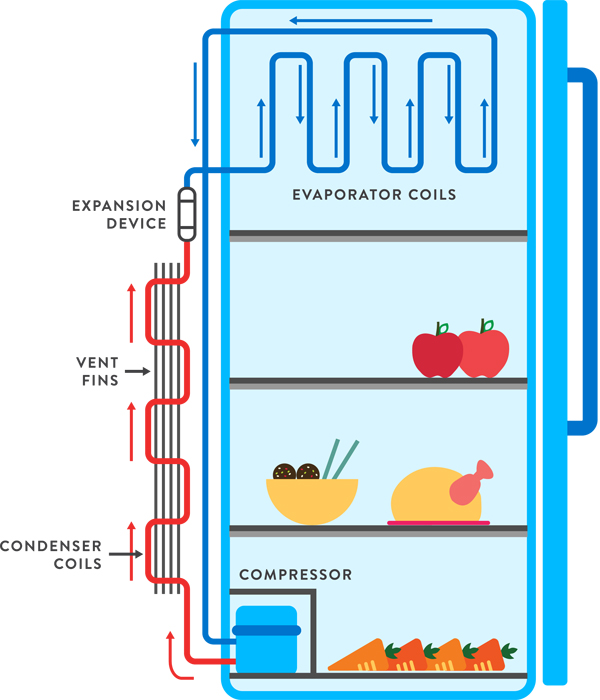
\includegraphics[width=0.45\textwidth]{Fridge.jpg}\pause&
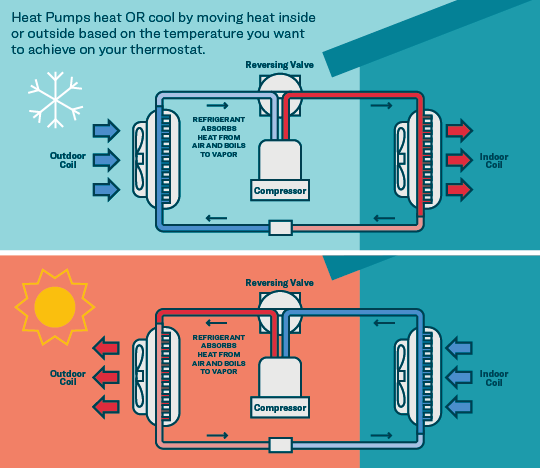
\includegraphics[width=0.45\textwidth]{heat-pump.png}
\end{tabular}
\end{frame}
\begin{frame}
\frametitle{Where do we apply thermal physics?}
\center
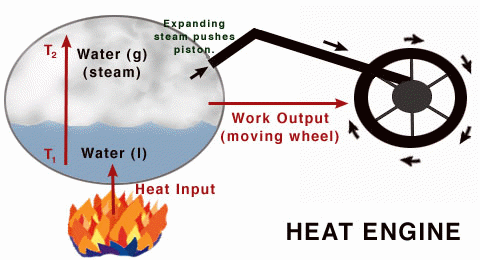
\includegraphics[width=0.8\textwidth]{RHE.png}
\end{frame}
\begin{frame}
\frametitle{Thermal Energy}
\center
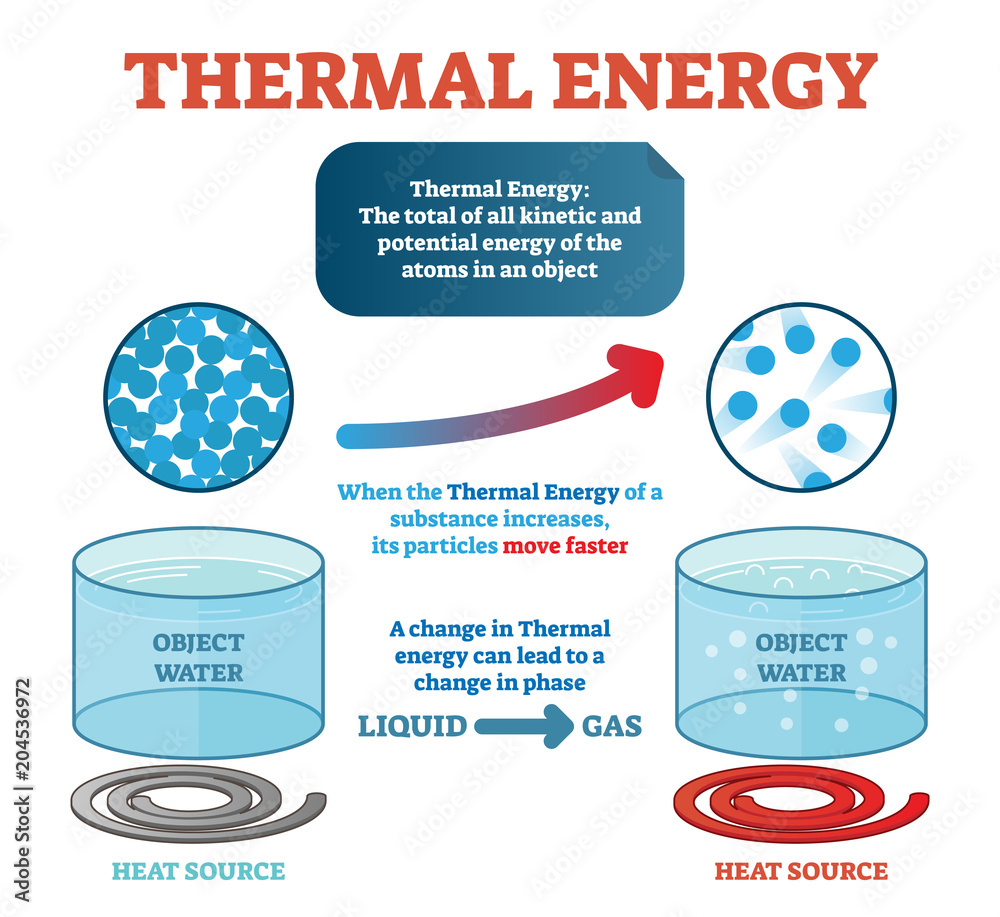
\includegraphics[width=0.7\textwidth]{thermal-energy.jpg}
\end{frame}
\begin{frame}
\frametitle{Temperature}
What is temperature?\pause

Mental Experiments:

\center
1. How do you feel?
\begin{tabular}{cc}
\onslide<2->{
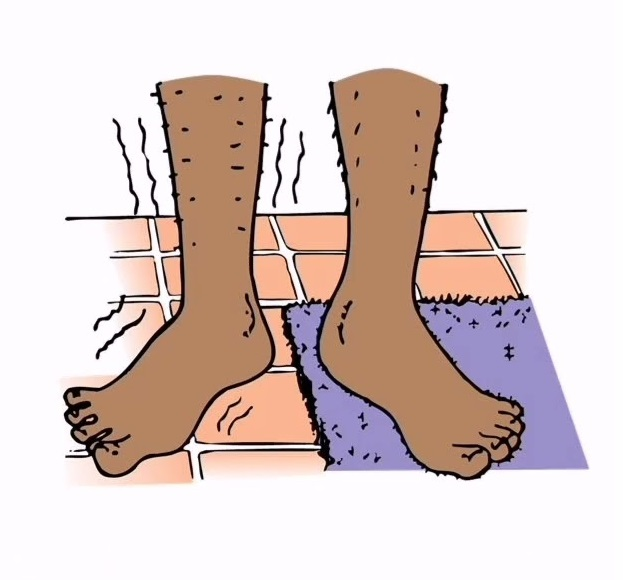
\includegraphics[width=0.45\textwidth]{carpet-vs-tile.jpg}
}&
\onslide<3->{

\includegraphics[width=0.45\textwidth]{fan.png}
}
\end{tabular}

\end{frame}
\begin{frame}
\frametitle{Temperature}
What is temperature?

Mental Experiments:

\center
2. Which one will boil quicker?
\vspace{\stretch{1}}

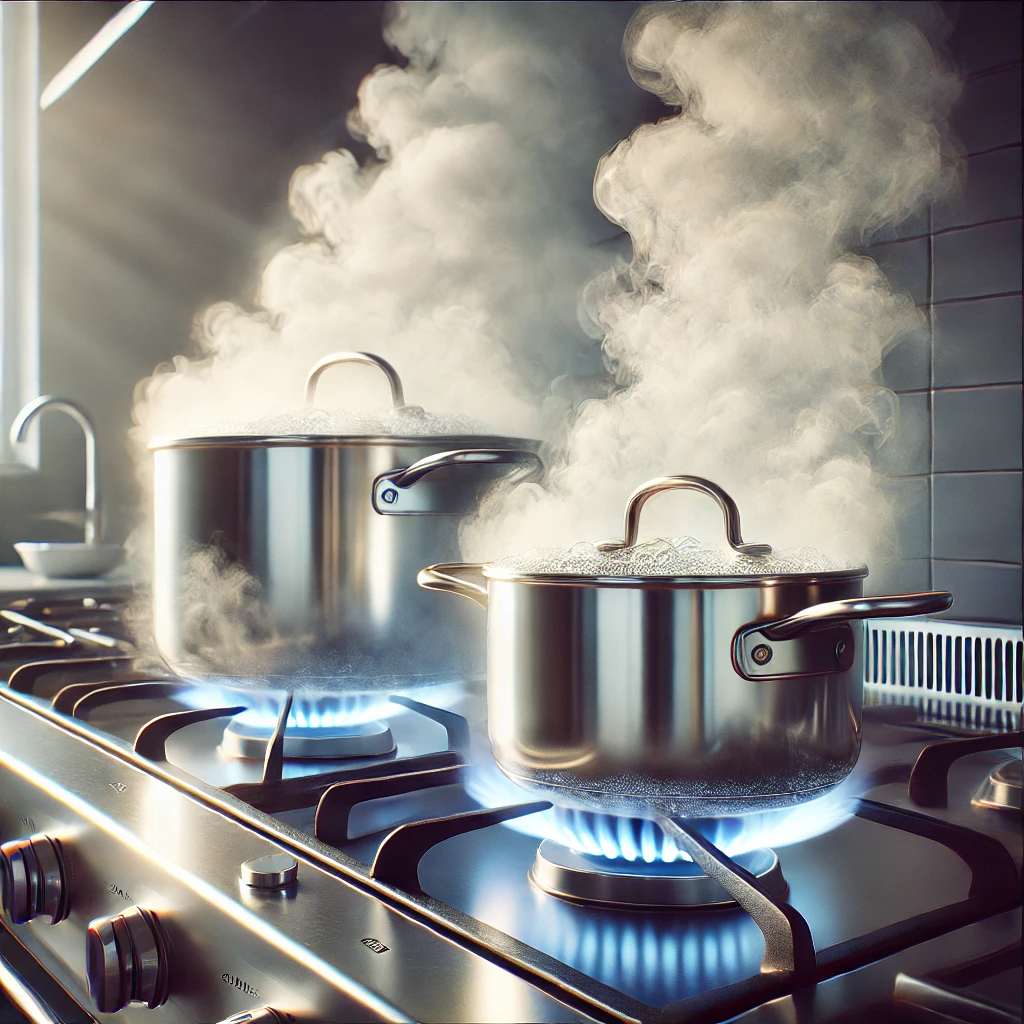
\includegraphics[width=.5\textwidth]{two-pots.png}

\end{frame}
\begin{frame}
\frametitle{Temperature}
What is temperature?

Mental Experiments:

\center
3. What will happen to the water?
\vspace{\stretch{1}}

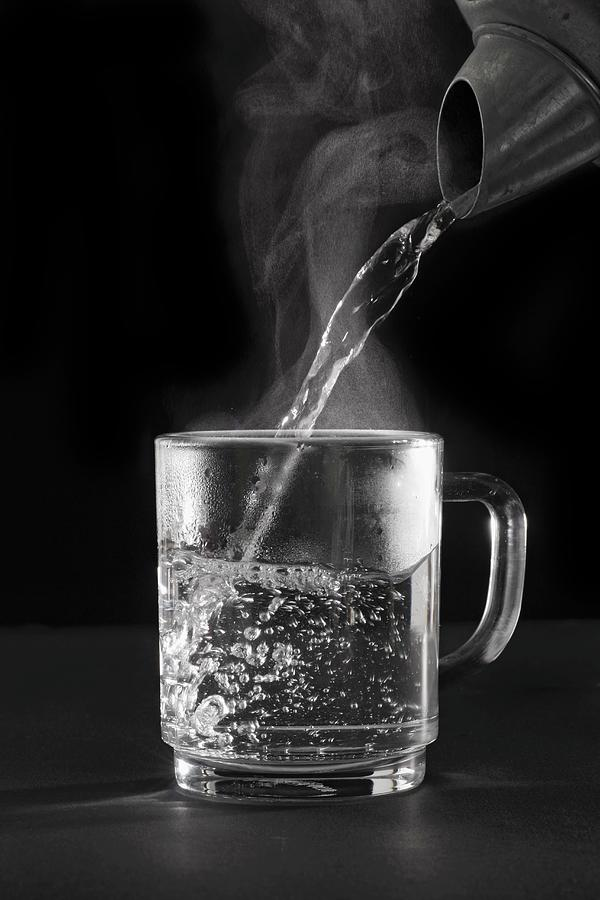
\includegraphics[width=.35\textwidth]{hot-water.jpg}
\end{frame}

\begin{frame}
\frametitle{Temperature}
In summary:
\begin{itemize}
\item
Temperature is the property that determines whether or not energy will transfer between two objects when they are in thermal contact.\pause
\item For a single object, the higher its temperature is, the more thermal energy it has.
\end{itemize}
\end{frame}

\begin{frame}
\frametitle{Temperature Scales: Celsius, Fahrenheit, and Kelvin}
What is the ice point and the steam point of water at atmospheric pressure?

\begin{center}
\begin{tabular}{ccc}
\ & Celsius& Fahrenheit\\[12pt]
ice point&\onslide<3->{$0^{\circ}C$}&\onslide<2->{$32^{\circ}F$}\\[12pt]
steam point&\onslide<3->{$100^{\circ}C$}&\onslide<2->{$212^{\circ}F$}
\end{tabular}
\end{center}

\onslide<4->{{\bf Exercise.} Convert the following temperatures to their values on the Fahrenheit scale: (a) the sublimation point of dry ice, $-78.5^{\circ}C$; (b) human body temperature, $37.0^{\circ}C$.}
\end{frame}

\begin{frame}
\frametitle{Temperature Scales: Celsius, Fahrenheit, and Kelvin}
Pressure v.s. Temperature

\begin{center}
\begin{tabular}{cc}

\includegraphics[width=.45\textwidth]{tire-pressure.png}
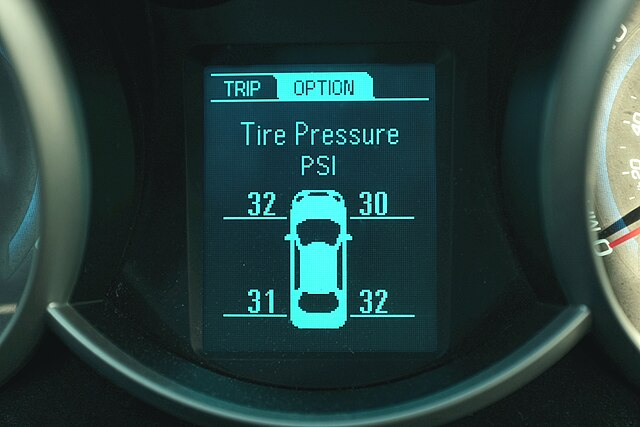
\includegraphics[width=.45\textwidth]{tire-pressure-meter.jpg}
\end{tabular}
\end{center}
\end{frame}


\begin{frame}
\frametitle{Temperature Scales: Celsius, Fahrenheit, and Kelvin}
The Kelvin Scale

\begin{center}
\begin{tabular}{c}
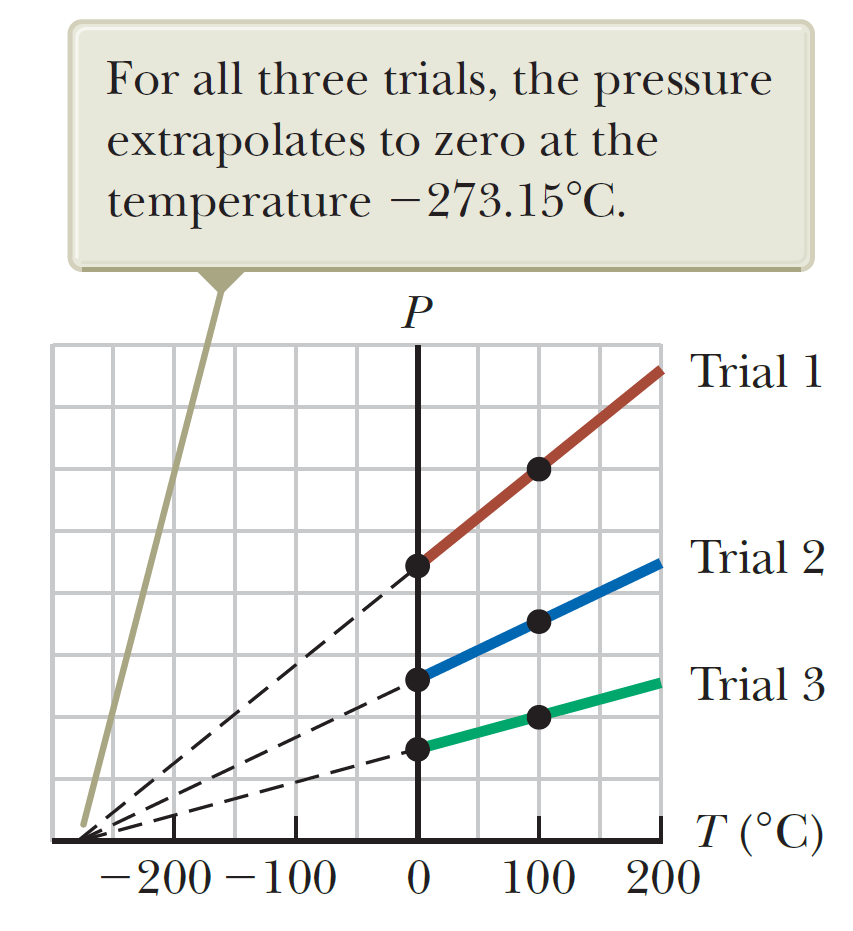
\includegraphics[width=0.5\textwidth]{Kelvin.png}
\end{tabular}
\pause
\[
Kelvin = Celsius + 273.15
\]
\end{center}
\end{frame}

\begin{frame}
\frametitle{Temperature Scales: Celsius, Fahrenheit, and Kelvin}
Examine the following report, extrapolate the temperature when the pressure is zero, and express the result in Kelvin scale.

Report: \href{./Pressure-Volume-Temperature Data for Oxygen.pdf}{Pressure-Volume-Temperature Data for Oxygen}
\end{frame}

\begin{frame}
\frametitle{Thermometer}
\begin{tabular}{cc}
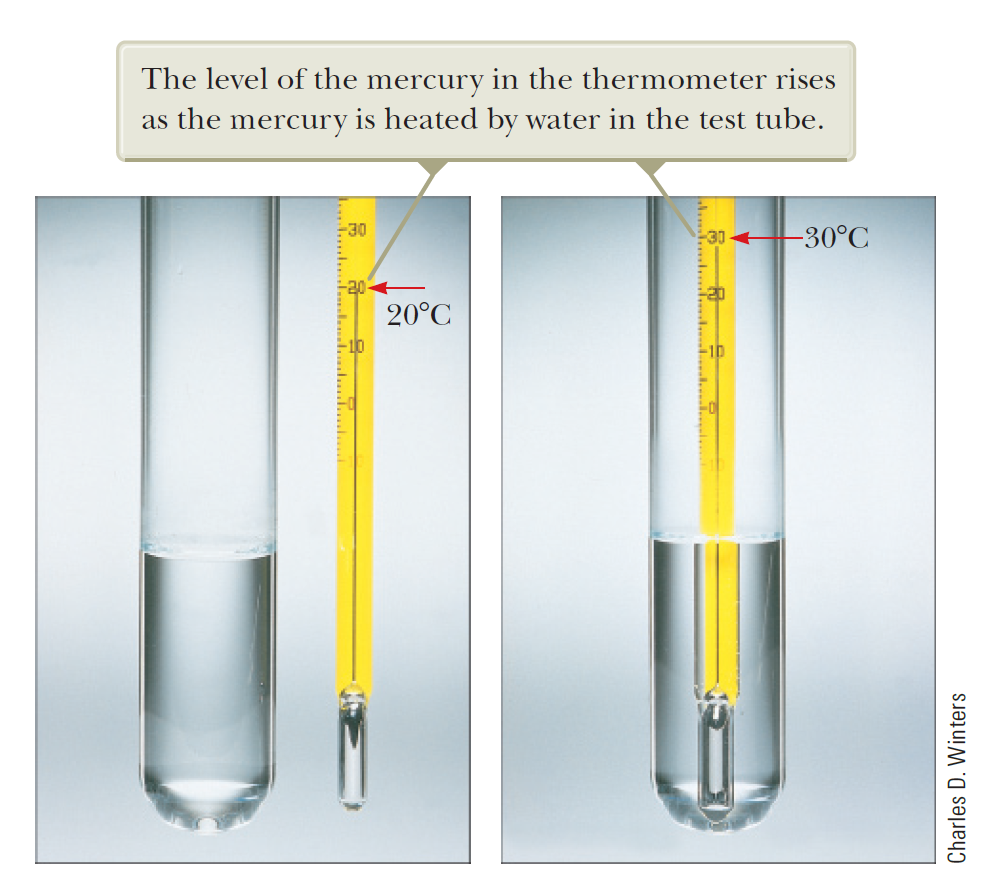
\includegraphics[width=0.45\textwidth]{mercury-thermometer.png}&\pause
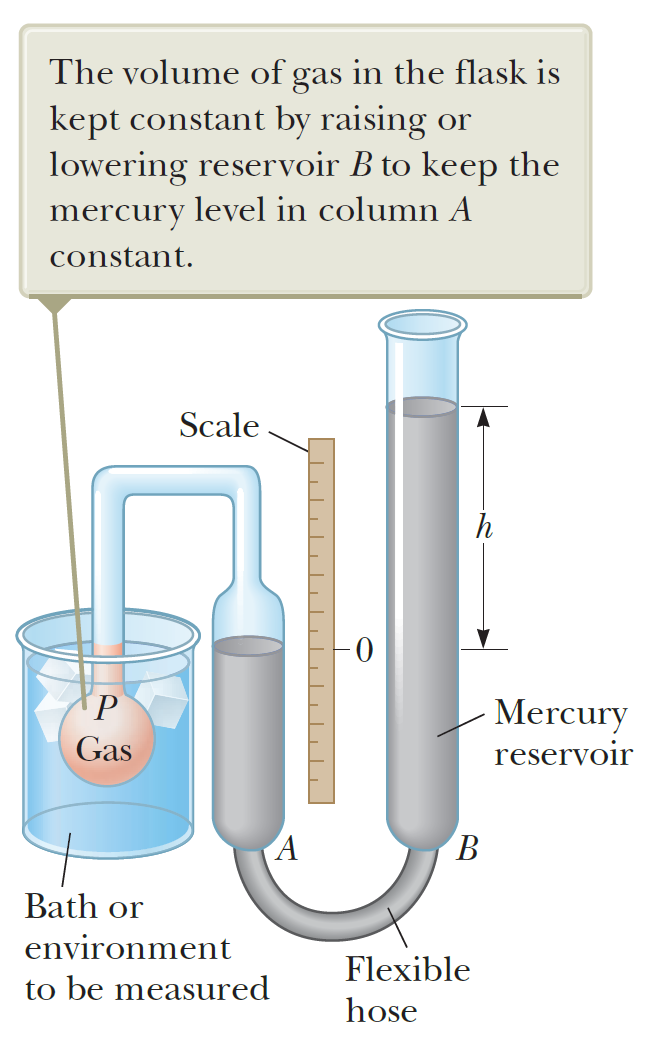
\includegraphics[width=0.45\textwidth]{constant-volume-thermometer.png}
\end{tabular}
\end{frame}

\end{document}